\documentclass[conference,onecolumn]{IEEEtran}

\usepackage[T1]{fontenc}
\usepackage[utf8]{inputenc}
\usepackage[spanish,es-tabla]{babel}
\usepackage{lmodern}
\usepackage{microtype}
\usepackage{csquotes}
\usepackage{amsmath,amssymb}
\usepackage{booktabs}
\usepackage{float}
\usepackage{tabularx}
\usepackage{array}
\usepackage{longtable}
\usepackage{graphicx}
\usepackage{pdflscape}
\usepackage{url}
\usepackage[hidelinks]{hyperref}
\usepackage[backend=biber,style=ieee,sorting=none]{biblatex}
\addbibresource{referencias.bib}
\AtBeginDocument{\spanishplainpercent}

\newcolumntype{Y}{>{\raggedright\arraybackslash}X}
\newcolumntype{L}[1]{>{\raggedright\arraybackslash}p{#1}}
\renewcommand{\IEEEkeywordsname}{Palabras clave}

\title{PE1: Ingeniería de Requisitos y Proceso de Requisitos aplicados al Sistema de gestión para un restaurante con IA}
\author{\IEEEauthorblockN{Arteaga Alava Danela Dayana, Chavarría Cuenca Tahiny Mel,\\
Naranjo Alfonzo Anthony Alexander}
\IEEEauthorblockA{Grupo ACNN · Carrera de Software\\
Facultad de Ciencias de la Computación\\
Universidad Técnica Estatal de Quevedo, Ecuador\\
Ingeniería de Requerimientos -- ISR-401}}

% Numeración arábiga como en la guía (0, 2, 2.1...)
\renewcommand{\thesection}{\arabic{section}}
\renewcommand{\thesubsection}{\thesection.\arabic{subsection}}
\renewcommand{\thesubsubsection}{\thesubsection.\arabic{subsubsection}}

\begin{document}
\maketitle
% Orden de las fuentes obligatorias según la guía: [1] a [10]
\nocite{ieee29148,iso15288,iso12207,iso25010,pohl2025,swebok2024,pmbok7,ireb31,moore2014,mavin2009}

\section*{Datos generales}
\begin{table}[H]
\centering\footnotesize
\begin{tabularx}{\textwidth}{@{}p{0.25\textwidth}Y@{}}
\toprule
\textbf{Campo} & \textbf{Detalle}\\
\midrule
Asignatura & Ingeniería de Requerimientos (ISR-401) · 4.\textsuperscript{o} nivel · Paralelo B\\
Práctica & PE1 · Práctica experimental de la Unidad 1\\
Grupo & ACNN\\
Integrantes y roles & Arteaga Alava Danela Dayana (Analista Líder, Investigador A y Documentador), Chavarría Cuenca Tahiny Mel (Investigador B), Naranjo Alfonzo Anthony Alexander (Investigador C)\\
Docente & Gleiston Cicerón Guerrero Ulloa, PhD\\
Sistema del PFC & Sistema de gestión para un restaurante con IA\\
Fecha de cierre & Domingo 15 de noviembre de 2026, 23:59\\
Repositorio & \url{https://github.com/darteagaa-boop/ISR401-GrupoACNN}\\
\bottomrule
\end{tabularx}
\end{table}

\tableofcontents

\setcounter{section}{-1}
\section{Sistema del Proyecto Fin de Curso}
% Responsable: Danela · Ronda 1 (viernes 13, hasta 21:00)
% Paso 1: c) descripción del PFC (máx. 150 palabras), d) 5 stakeholders con la matriz poder/interés [7], e) tipo de sistema y su justificación.



\setcounter{section}{1}
\section{Fundamento teórico}
% Responsable: Danela · Ronda 2 (sábado 14, hasta 13:00)
\subsection{Definición y tipos de requisitos}
\subsubsection{Requisito}

\textbf{Definición:} Un requisito es un enunciado que expresa una necesidad junto con las restricciones y condiciones que la acompañan \cite[\nopp cl.~3.1.19]{ieee29148}. El IREB distingue sentidos del término, una necesidad percibida por un stakeholder, una capacidad o propiedad que el sistema debe tener, y la representación documentada de cualquiera de las dos \cite{ireb31}.

\textbf{Explicación:} Un requisito no es solo una función deseada, sino una necesidad expresada de forma que el equipo pueda construirla y comprobarla. Por eso la definición incluye las condiciones y restricciones, que dicen cuándo y cómo se aplica. Distinguir los tres sentidos del IREB ayuda a entender que una necesidad que solo existe en la cabeza del cliente todavía no es un requisito documentado.

\textbf{Ejemplo en El Balcón Restaurant:} El propietario necesita saber qué insumos comprar cada día. Esa necesidad se convierte en un requisito cuando se documenta, por ejemplo: “El sistema deberá sugerir la lista de compras del día siguiente a partir de la demanda estimada de cada plato”.

\subsubsection{Stakeholder}

\textbf{Definición:} Un stakeholder es una persona u organización que tiene un derecho, una participación o un interés en el sistema que este satisfaga sus necesidades y expectativas \cite[\nopp cl.~3.1.28]{ieee29148}.

\textbf{Explicación:} Los requisitos nacen de los stakeholders, por lo que identificarlos es el primer paso del proceso. No todos son usuarios del sistema, porque también cuentan quienes lo financian o lo regulan. Olvidar a un stakeholder suele significar olvidar los requisitos que solo él conoce.

\textbf{Ejemplo en El Balcón Restaurant:} Además de los meseros y clientes, el SRI es un stakeholder de El Balcón Restaurant aunque nunca use el sistema, sus normas de facturación electrónica imponen requisitos (Sección 0).

\subsubsection{Restricción}

\textbf{Definición:} Una restricción es una limitación impuesta desde fuera sobre el sistema, su diseño, su implementación o el proceso con el que se desarrolla \cite[\nopp cl.~3.1.7]{ieee29148}.

\textbf{Explicación:} A diferencia de un requisito funcional, una restricción no describe lo que el sistema hace, sino los límites dentro de los cuales debe construirse. Suele venir de leyes, presupuestos, tecnologías existentes o decisiones del cliente. Reconocerla a tiempo evita diseñar soluciones que luego no se pueden usar.

\textbf{Ejemplo en El Balcón Restaurant:} El restaurante ya usa tablets Android para tomar pedidos, por lo que una restricción es que la aplicación de los meseros funcione en esos dispositivos.

\subsubsection{Requisitos de producto y requisitos de proceso}

\textbf{Definición:} La norma describe los requisitos de proceso como exigencias de los stakeholders, normalmente del usuario, impuestas mediante el contrato o el cumplimiento de leyes o directivas de trabajo \cite[\nopp cl.~5.2.8.3]{ieee29148}. Los requisitos de producto, en cambio, describen lo que debe hacer o cumplir el sistema.

\textbf{Explicación:} La diferencia está en el objeto del requisito, del producto que se entrega o la forma de construirlo. Un requisito de producto se verifica probando el sistema, mientras que uno de proceso se verifica revisando cómo se trabajó. Mezclarlos en la misma lista confunde las pruebas, por eso conviene identificar su tipo desde el inicio.

\textbf{Ejemplo en El Balcón Restaurant:} “El sistema deberá registrar el cierre de caja diario” es un requisito de producto. “Cada entrega se validará con el propietario antes de instalarse en el restaurante” es un requisito de proceso.

\subsubsection{Tipos de requisitos}

\textbf{Definición:} La norma recomienda registrar el tipo de cada requisito como un atributo, porque los requisitos varían en su intención y en las propiedades que representan, e incluye como ejemplo los tipos funcional y de rendimiento, de interfaz, de proceso, no funcional, de usabilidad y de factores humanos \cite[\nopp cl.~5.2.8.3]{ieee29148}. El IREB y Pohl agrupan los requisitos en funcionales, de calidad y restricciones \cite{pohl2025,ireb31}.

\textbf{Explicación:} Clasificar los requisitos por tipo permite repartirlos, analizarlos y verificarlos con la técnica adecuada para cada uno. Las dos clasificaciones no se contradicen, porque la del IREB es más general y la de la norma detalla subtipos. En el sistema del restaurante se usarán ambas, la del IREB para la clasificación principal y la de la norma para el atributo de tipo de cada requisito.

\textbf{Ejemplo en El Balcón Restaurant:} La siguiente tabla muestra un ejemplo de cada tipo.

\begin{table}[H]
\centering\footnotesize
\caption{Tipos de requisitos según IEEE 29148 con ejemplos en El Balcón Restaurant}\label{tab:tipos-requisitos}
\begin{tabularx}{\textwidth}{@{}p{0.22\textwidth}Yp{0.36\textwidth}@{}}
\toprule
\textbf{Tipo según IEEE 29148} & \textbf{Qué expresa} & \textbf{Ejemplo en El Balcón Restaurant}\\
\midrule
\textbf{Funcional / rendimiento} & Funciones o tareas que realiza el sistema, y qué tan bien las realiza & El sistema enviará cada pedido de mesa a la pantalla de cocina\\
\textbf{Interfaz} & Cómo interactúa el sistema con sistemas externos o entre sus elementos & Conexión con el sistema de facturación electrónica del SRI\\
\textbf{Proceso} & Exigencias sobre cómo se desarrolla el sistema, impuestas por contrato, leyes o políticas & El propietario aprobará cada entrega antes de pasar a producción\\
\textbf{Calidad (no funcional)} & Propiedades como seguridad, fiabilidad o mantenibilidad, con sus medidas & Disponibilidad del sistema durante el horario de atención\\
\textbf{Usabilidad / calidad en uso} & Eficacia, eficiencia y satisfacción del usuario en su contexto de uso & Un mesero nuevo registra un pedido sin capacitación previa\\
\textbf{Factores humanos} & Resultados de la interacción con las personas, como seguridad o bienestar & Pantallas legibles en la cocina, con calor y poca distancia de lectura\\
\bottomrule
\end{tabularx}
\end{table}

\subsubsection{Glosario de términos base}\mbox{}

\begin{table}[H]
\centering\footnotesize
\caption{Glosario de términos base}\label{tab:glosario}
\begin{tabularx}{\textwidth}{@{}p{0.22\textwidth}Yp{0.14\textwidth}@{}}
\toprule
\textbf{Término} & \textbf{Definición en la norma} & \textbf{Cláusula}\\
\midrule
\textbf{Requisito} & Enunciado que traduce o expresa una necesidad junto con sus restricciones y condiciones asociadas & \cite[\nopp cl.~3.1.19]{ieee29148}\\
\textbf{Stakeholder} & Persona u organización con un derecho, participación, reclamo o interés en el sistema o en que cumpla sus necesidades & \cite[\nopp cl.~3.1.28]{ieee29148}\\
\textbf{Restricción} & Limitación impuesta desde fuera sobre el sistema, su diseño, su implementación o su proceso de desarrollo & \cite[\nopp cl.~3.1.7]{ieee29148}\\
\textbf{Verificación} & Confirmación con evidencia objetiva de que se cumplieron los requisitos especificados & \cite[\nopp cl.~3.1.37]{ieee29148}\\
\textbf{Validación} & Confirmación con evidencia objetiva de que se cumplieron los requisitos para el uso previsto & \cite[\nopp cl.~3.1.36]{ieee29148}\\
\bottomrule
\end{tabularx}
\end{table}

% Responsable: Danela · Ronda 3 (sábado 14, hasta 21:00)
\subsection{Requisitos funcionales y no funcionales}
\subsubsection{Requisito funcional}

\textbf{Definición:} Los requisitos funcionales describen las funciones o tareas que debe realizar el sistema o uno de sus elementos \cite[\nopp cl.~5.2.8.3]{ieee29148}.

\textbf{Explicación:} Un requisito funcional responde a la pregunta de qué hace el sistema. Se expresa con una acción observable que se puede probar con un caso de uso o un escenario, si se elimina un requisito funcional, el sistema pierde una capacidad concreta.

\textbf{Ejemplo en El Balcón Restaurant:} “Cuando el mesero confirme un pedido, el sistema deberá enviarlo a la pantalla de cocina” es un requisito funcional de El Balcón Restaurant.

\subsubsection{Requisito no funcional o de calidad}

\textbf{Definición:} Los requisitos de calidad, también llamados no funcionales, expresan propiedades como la fiabilidad, la mantenibilidad o la seguridad, y deben incluir sus medidas cuando corresponda \cite[\nopp cl.~5.2.8.3]{ieee29148}. Para clasificarlos se usa el modelo de calidad de producto de ISO/IEC 25010:2023 \cite{iso25010}. Glinz señala que el término “no funcional” se usa de forma poco precisa y propone tratarlos según la propiedad que expresan \cite{glinz2007}.

\textbf{Explicación:} Un requisito no funcional responde a la pregunta de qué tan bien hace el sistema lo que hace. Por eso no agrega funciones, sino que pone condiciones de calidad sobre las funciones existentes. Si no se cuantifica, queda abierto a interpretaciones y no se puede verificar.

\textbf{Ejemplo en El Balcón Restaurant:} “El sistema debe ser rápido” no es verificable. Su versión cuantificada sería: “El 95 \% de los pedidos deberá aparecer en la pantalla de cocina en 3 segundos o menos desde que el mesero los confirma”.

\subsubsection{Requisito de rendimiento}

\textbf{Definición:} La norma considera el rendimiento como un atributo de una función, que normalmente se expresa de forma cuantitativa, y advierte que un requisito de rendimiento por sí solo es incompleto \cite[\nopp cl.~5.2.8.3]{ieee29148}.

\textbf{Explicación:} Un requisito de rendimiento siempre se refiere a una función concreta, porque mide qué tan rápido o cuánto la realiza. Por eso debe redactarse ligado a esa función y no de forma aislada, porque expresarlo con números permite comprobarlo con pruebas de carga o mediciones.

\textbf{Ejemplo en El Balcón Restaurant:} El requisito de los 3 segundos de la cocina está ligado a la función de enviar pedidos. Otro ejemplo es que la sugerencia de compras de la IA se genere antes de las 22:00, al cerrar la cena.

\subsubsection{Diferencia entre funcional y no funcional y su lugar en el ERS}

\textbf{Definición:} En la especificación de requisitos de software, la norma organiza los requisitos especificados en interfaces externas, funciones, usabilidad, rendimiento, base de datos lógica, restricciones de diseño, cumplimiento de estándares y atributos del sistema de software \cite[\nopp cl.~9.6.10–9.6.18]{ieee29148}, y dedica un apartado a la verificación de cada requisito \cite[\nopp cl.~9.6.19]{ieee29148}.

\textbf{Explicación:} La estructura del ERS muestra que los requisitos funcionales y los no funcionales se documentan por separado, pero se relacionan entre sí. Los atributos de calidad como fiabilidad, disponibilidad o seguridad se especifican aparte para que cada uno tenga su medida.

\textbf{Ejemplo en El Balcón Restaurant:} En el ERS de El Balcón Restaurant, el envío de pedidos a cocina va en funciones, el tiempo de 3 segundos en rendimiento, la conexión con el SRI en interfaces externas y la protección de los datos de los clientes en atributos del sistema. En verificación se indicaría, por ejemplo, que el tiempo se mide con 100 pedidos de prueba.

% Responsable: Tahiny · Ronda 1 (viernes 13, hasta 21.00)
% Para cada concepto: (i) definición formal con cita IEEE comprimida, (ii) explicación propia de mínimo 3 oraciones, (iii) ejemplo del Sistema de gestión para un restaurante con IA.
\subsection{Requisitos de sistema y requisitos de software}

% Responsable: Tahiny · Ronda 2 (sábado 14, hasta 13.00)
% Para cada concepto: (i) definición formal con cita IEEE comprimida, (ii) explicación propia de mínimo 3 oraciones, (iii) ejemplo del Sistema de gestión para un restaurante con IA.
\subsection{Modelo de calidad ISO/IEC 25010:2023}

La calidad de un sistema no se especifica con adjetivos como ``r\'apido'' o ``seguro'', sino con un modelo que defina qu\'e propiedades se miden. ISO/IEC 25010:2023 ofrece ese modelo para el producto de software y de sistemas \cite{iso25010}.

\subsubsection{El modelo de calidad del producto y sus nueve caracter\'isticas}
\textbf{(i) Definici\'on formal.} ISO/IEC 25010:2023 define un modelo de calidad del producto compuesto por nueve caracter\'isticas, cada una dividida en subcaracter\'isticas: idoneidad funcional, eficiencia de desempe\~no, compatibilidad, capacidad de interacci\'on, fiabilidad, seguridad, mantenibilidad, flexibilidad y protecci\'on (\emph{safety}) \cite{iso25010}.
\par
\textbf{(ii) Explicaci\'on propia.} El modelo funciona como un vocabulario com\'un: cuando alguien pide ``que el sistema sea confiable'', el equipo puede preguntar a cu\'al subcaracter\'istica se refiere (disponibilidad, tolerancia a fallos, recuperabilidad) y c\'omo se medir\'a. En esta edici\'on, la antigua usabilidad pas\'o a llamarse capacidad de interacci\'on y se a\~nadieron flexibilidad y protecci\'on. Usar el modelo evita olvidar dimensiones de calidad y facilita acordar con el cliente qu\'e importa m\'as.\par
\textbf{(iii) Ejemplo en El Balc\'on.} La Tabla~\ref{tab:iso} aplica las nueve caracter\'isticas a El Balc\'on e indica qu\'e requisito de la Tabla~\ref{tab:requisitos} cubre cada una.\par

\begin{table}[ht]
\centering
\small
\caption{Caracter\'isticas de ISO/IEC 25010:2023 aplicadas al SGR-IA de El Balc\'on \cite{iso25010}.}
\label{tab:iso}
\begin{tabular}{@{}>{\raggedright\arraybackslash}p{2.6cm}>{\raggedright\arraybackslash}p{4.3cm}>{\raggedright\arraybackslash}p{5.2cm}>{\raggedright\arraybackslash}p{2.2cm}@{}}
\toprule
\textbf{Caracter\'istica} & \textbf{Subcaracter\'isticas} & \textbf{Qu\'e significa en El Balc\'on} & \textbf{Requisito} \\
\midrule
Idoneidad funcional & Completitud, correcci\'on y pertinencia funcional & El pron\'ostico de demanda debe acertar lo suficiente para decidir las compras & RNF-05 \\
Eficiencia de desempe\~no & Comportamiento temporal, uso de recursos, capacidad & Respuesta r\'apida del estado de pedidos en hora pico & RNF-01 \\
Compatibilidad & Coexistencia, interoperabilidad & Intercambio de comprobantes con el servicio web del SRI & RI-02 \\
Capacidad de interacci\'on & Reconocibilidad, aprendizaje, operabilidad, protecci\'on ante errores del usuario, entre otras & Un mesero nuevo aprende a tomar pedidos con poca capacitaci\'on & RNF-04 \\
Fiabilidad & Ausencia de fallos, disponibilidad, tolerancia a fallos, recuperabilidad & El sistema funciona durante todo el horario de atenci\'on de El Balc\'on & RNF-03 \\
Seguridad & Confidencialidad, integridad, no repudio, responsabilidad, autenticidad, resistencia & Acceso por rol y protecci\'on de los datos de los clientes & RNF-02, RCF-01 \\
Mantenibilidad & Modularidad, reusabilidad, analizabilidad, modificabilidad, testeabilidad & Cambiar el men\'u o la tarifa de IVA sin reescribir el sistema & No priorizada \\
Flexibilidad & Adaptabilidad, escalabilidad, instalabilidad, reemplazabilidad & Abrir un segundo local con la misma plataforma & No priorizada \\
Protecci\'on (\emph{safety}) & Restricci\'on operacional, identificaci\'on de riesgos, seguridad ante fallos, advertencia de peligros, integraci\'on segura & El sistema no controla equipos de cocina & No aplica \\
\bottomrule
\end{tabular}
\end{table}

\subsubsection{Calidad y requisitos no funcionales}
\textbf{(i) Definici\'on formal.} Los requisitos no funcionales, llamados requisitos de calidad por Pohl, expresan qu\'e tan bien debe cumplir el sistema sus funciones \cite{pohl2025}; Glinz advierte que el t\'ermino ``no funcional'' se ha definido de formas inconsistentes y que conviene precisar cada requisito \cite{glinz2007}.\par
\textbf{(ii) Explicaci\'on propia.} El modelo de calidad aporta la categor\'ia del requisito y la m\'etrica lo hace verificable. Un requisito de calidad bien formado indica la caracter\'istica, la medida, el umbral y las condiciones de uso. Sin esos elementos, cada persona del equipo interpretar\'ia el requisito a su manera y no habr\'ia forma de probarlo.\par
\textbf{(iii) Ejemplo en El Balc\'on.} ``El sistema debe ser r\'apido'' se reescribe como RNF-01: el 95\,\% de las consultas de estado de pedidos debe responder en menos de 2 segundos con 50 usuarios concurrentes. La caracter\'istica es eficiencia de desempe\~no, la medida es el tiempo de respuesta, el umbral es 2 segundos y la condici\'on es la carga de 50 usuarios.\par

\subsubsection{Selecci\'on de caracter\'isticas relevantes}
\textbf{(i) Criterio del equipo.} En este proyecto se seleccionan las caracter\'isticas relevantes seg\'un el contexto de uso y las necesidades de los stakeholders. Esta selecci\'on es una decisi\'on del equipo para delimitar el alcance del SGR-IA.
\par
\textbf{(ii) Explicaci\'on propia.} Especificar las nueve caracter\'isticas con el mismo detalle ser\'ia costoso y poco realista en un proyecto de un semestre. Lo recomendable es priorizar las que afectan directamente al negocio y justificar las que se dejan fuera. Esa justificaci\'on tambi\'en es parte del an\'alisis de requisitos, porque deja claro qu\'e se decidi\'o no especificar.\par
\textbf{(iii) Ejemplo en El Balc\'on.} Se priorizaron cinco caracter\'isticas: desempe\~no, seguridad, fiabilidad, capacidad de interacci\'on e idoneidad funcional, m\'as la compatibilidad con el SRI. Mantenibilidad y flexibilidad quedan para una versi\'on posterior, y protecci\'on no aplica porque el sistema no controla equipos de cocina.\par

% Responsable: Anthony · Ronda 1 (viernes 13, hasta 21.00)
% Para cada concepto: (i) definición formal con cita IEEE comprimida, (ii) explicación propia de mínimo 3 oraciones, (iii) ejemplo del Sistema de gestión para un restaurante con IA.
\subsection{Tipos de sistemas}
La clasificación de un sistema permite identificar su propósito, su entorno
de operación y la relación que mantiene con las personas y otros elementos
externos. En Ingeniería de Requisitos esta caracterización ayuda a establecer
el alcance del producto y a comprender las necesidades de los stakeholders
antes de especificar las funciones concretas del software
\cite{ieee29148,pohl2025}.

\subsubsection{Sistema de información de gestión}

\textbf{(i) Definición formal.}
Un sistema de información permite registrar, almacenar, procesar y comunicar
datos con el propósito de apoyar las actividades de una organización. Desde
la perspectiva de Ingeniería de Requisitos, sus funciones deben responder a
las necesidades de los stakeholders y al contexto en el que será utilizado
\cite{ieee29148,pohl2025}.

\textbf{(ii) Explicación propia.}
Este tipo de sistema trabaja principalmente con información generada durante
las actividades de una organización. Su objetivo no consiste únicamente en
guardar datos, sino también en procesarlos para facilitar las operaciones y
apoyar la toma de decisiones. Por esta razón, sus requisitos deben establecer
qué información se registra, quién puede utilizarla y qué resultados debe
proporcionar el sistema.

\textbf{(iii) Aplicación al PFC.}
El Sistema de gestión para un restaurante con IA desarrollado para
El Balcón Restaurant, en Quevedo, se clasifica principalmente como un sistema
de información de gestión. La aplicación registrará y procesará información
relacionada con pedidos, reservas, menú, inventario, ventas y cierre de caja.
Estos datos permitirán apoyar las actividades diarias del restaurante y
servirán también como fuente para las funcionalidades de inteligencia
artificial definidas en el proyecto.

\subsubsection{Sistema sociotécnico}

\textbf{(i) Definición formal.}
El análisis de requisitos debe considerar no solamente los componentes de
software, sino también a las personas, los procesos organizacionales y el
entorno en el que funcionará el sistema. Esta interacción entre elementos
humanos y tecnológicos caracteriza a los sistemas sociotécnicos
\cite{pohl2025,swebok2024}.

\textbf{(ii) Explicación propia.}
El funcionamiento correcto de una aplicación empresarial no depende
exclusivamente del código desarrollado. Los usuarios realizan actividades,
siguen procedimientos y toman decisiones que influyen directamente en los
resultados obtenidos mediante el sistema. Por ello, durante la Ingeniería de
Requisitos es necesario comprender tanto la parte tecnológica como la forma
real en que trabajan las personas dentro de la organización.

\textbf{(iii) Aplicación al PFC.}
El sistema de El Balcón Restaurant posee una naturaleza sociotécnica porque
en sus procesos intervienen el propietario, el jefe de cocina, los meseros,
el cajero y los clientes. Por ejemplo, el mesero registra un pedido, cocina
recibe la información para preparar los platos y posteriormente el cajero
utiliza los datos registrados para realizar el cobro. El resultado final
depende de la interacción entre los usuarios, los procedimientos internos
del restaurante y la aplicación.

\subsubsection{Sistema con componente de inteligencia artificial}

\textbf{(i) Definición formal.}
Dentro del proyecto, la inteligencia artificial constituye un componente
integrado al sistema de información. Las capacidades incorporadas al software
deben originarse en necesidades identificadas y expresarse mediante requisitos
que puedan ser documentados y posteriormente validados
\cite{ieee29148,pohl2025}.

\textbf{(ii) Explicación propia.}
La incorporación de inteligencia artificial no cambia el propósito principal
del sistema, que continúa siendo gestionar información y procesos del
restaurante. La IA utiliza los datos disponibles para generar resultados que
sirven como apoyo a determinadas decisiones. En este proyecto sus resultados
se consideran recomendaciones, por lo que las personas mantienen la
responsabilidad sobre las decisiones finales.

\textbf{(iii) Aplicación al PFC.}
En El Balcón Restaurant se han definido dos funciones principales de
inteligencia artificial. La primera permitirá estimar la demanda diaria de
cada plato utilizando información histórica de ventas, con el objetivo de
apoyar la planificación de compras de insumos. La segunda permitirá recomendar
platos a los clientes tomando como referencia sus pedidos anteriores. En ambos
casos la inteligencia artificial funciona como apoyo y no como sustituto de
la decisión humana.

\subsubsection{Clasificación del PFC}

De acuerdo con las características identificadas, el proyecto se considera
principalmente un \textbf{sistema de información de gestión con un componente
de inteligencia artificial}. También presenta una naturaleza sociotécnica,
debido a que su funcionamiento depende de la interacción entre el software,
los usuarios y los procedimientos internos de El Balcón Restaurant.

El sistema no se considera embebido, ya que su función principal no consiste
en controlar directamente dispositivos físicos. Tampoco se clasifica como un
sistema crítico de seguridad, puesto que las funciones de inteligencia
artificial generan estimaciones y recomendaciones que posteriormente son
evaluadas por las personas responsables. Esta clasificación permite orientar
los requisitos hacia la gestión de información, la operación del restaurante
y el apoyo a la toma de decisiones.

% Responsable: Anthony · Ronda 2 (sábado 14, hasta 13.00)
% Para cada concepto: (i) definición formal con cita IEEE comprimida, (ii) explicación propia de mínimo 3 oraciones, (iii) ejemplo del Sistema de gestión para un restaurante con IA.
\subsection{Proceso de requisitos: framework de Pohl, modelos de proceso y contexto del sistema}


\section{Artefactos del procedimiento}
% Responsable: Tahiny · Ronda 3 (sábado 14, hasta 21.00)
% Paso 4 y rúbrica C1: mínimo 15 requisitos únicos con ID [ID | Tipo | Descripción | MoSCoW | Fuente] cubriendo negocio, stakeholder, usuario, funcional (EARS [10]), no funcional (ISO/IEC 25010:2023 [4]), interfaz (con su tipo), rendimiento, restricción y conformidad.
\subsection{Tabla de tipos de requisitos aplicada al PFC}

% Responsable: Danela · Adicional de la rúbrica · Ronda 4 (domingo 15, hasta 15.00)
% Rúbrica C2: evaluar cada uno de los 15 requisitos con las propiedades de IEEE 29148 (necesario, no ambiguo, verificable, trazable, etc.) con argumentación verificable.
\subsection{Evaluación de los requisitos con las propiedades de IEEE 29148}

% Responsable: Anthony · Ronda 3 (sábado 14, hasta 21.00)
% Paso 5: a) límite del sistema con mínimo 5 entidades externas (tipo de datos, protocolo y frecuencia), b) visión en formato Moore [9], c) ocho perspectivas de contexto [5] con 3 preguntas y 2 requisitos o restricciones cada una.
\subsection{Contexto del sistema y declaración de visión}

% Responsable: Anthony · Adicional de la rúbrica · Ronda 4 (domingo 15, hasta 15.00)
% Rúbrica C3: actores del proceso (ingeniero de requisitos, cliente, usuario, desarrollador) con roles concretos en el restaurante, y actividades centrales y transversales del framework de Pohl mapeadas al sistema.
\subsection{Actores del proceso y framework de IR aplicado}
\subsubsection{Actores del proceso de requisitos}

El proceso de Ingeniería de Requisitos requiere la participación de actores
con responsabilidades diferentes. Para el PFC se identifican los roles de
ingeniero de requisitos, cliente, usuario y desarrollador, relacionándolos
con el contexto concreto de El Balcón Restaurant
\cite{ieee29148,pohl2025}.

\begin{table}[H]
\centering
\footnotesize
\caption{Actores del proceso de requisitos aplicados al PFC}
\label{tab:actores-ir}
\begin{tabularx}{\textwidth}{@{}p{0.21\textwidth}p{0.28\textwidth}Y@{}}
\toprule
\textbf{Actor del proceso} &
\textbf{Representación en el PFC} &
\textbf{Responsabilidad} \\
\midrule

Ingeniero de requisitos &
Equipo ACNN &
Elicitar, analizar, documentar, negociar y validar las necesidades del
restaurante, manteniendo coherencia y trazabilidad entre los artefactos. \\

Cliente &
Propietario de El Balcón Restaurant &
Expresar objetivos y necesidades del negocio, establecer prioridades y
aprobar los requisitos y el alcance acordado. \\

Usuario &
Jefe de cocina, meseros, cajero y clientes &
Aportar información sobre los procesos reales, las tareas cotidianas, las
dificultades y las condiciones de uso que debe considerar el sistema. \\

Desarrollador &
Equipo técnico encargado de implementar el PFC &
Transformar los requisitos aprobados en componentes de software, mantener
trazabilidad con la especificación e informar restricciones técnicas que
puedan afectar la solución. \\

\bottomrule
\end{tabularx}
\end{table}

\subsubsection{Actividades centrales del framework de Pohl}

Pohl organiza las actividades centrales de Ingeniería de Requisitos en
elicitación, documentación y negociación \cite{pohl2025}. Estas actividades
se relacionan entre sí y pueden repetirse durante el proyecto cuando se
descubre nueva información o se modifican las necesidades.

\begin{table}[H]
\centering
\footnotesize
\caption{Actividades centrales de IR aplicadas a El Balcón}
\label{tab:actividades-centrales}
\begin{tabularx}{\textwidth}{@{}p{0.20\textwidth}YY@{}}
\toprule
\textbf{Actividad} &
\textbf{Aplicación en el restaurante} &
\textbf{Artefacto o resultado} \\
\midrule

Elicitación &
Obtener información del propietario y los usuarios acerca del registro de
pedidos, reservas, inventario, ventas y necesidades de apoyo mediante IA. &
Stakeholders, contexto, preguntas de análisis y candidatos a requisitos. \\

Documentación &
Representar de forma estructurada las necesidades obtenidas para que puedan
ser revisadas y utilizadas durante el desarrollo. &
Tabla de requisitos, descripción del sistema, límite, visión y perspectivas
de contexto. \\

Negociación &
Resolver diferencias de prioridad, alcance o interpretación entre el
propietario, usuarios y equipo del proyecto. &
Requisitos acordados, prioridades y decisiones de alcance. \\

\bottomrule
\end{tabularx}
\end{table}

\subsubsection{Actividades transversales}

La validación y la gestión son actividades transversales porque acompañan a
las actividades centrales y a los artefactos producidos durante el proceso
\cite{pohl2025}.

\begin{table}[H]
\centering
\footnotesize
\caption{Actividades transversales aplicadas al PFC}
\label{tab:actividades-transversales}
\begin{tabularx}{\textwidth}{@{}p{0.20\textwidth}YY@{}}
\toprule
\textbf{Actividad} &
\textbf{Aplicación en El Balcón} &
\textbf{Resultado esperado} \\
\midrule

Validación &
Revisar con el cliente y los usuarios que los requisitos representen las
necesidades reales y evaluar que sean claros, verificables y coherentes. &
Corrección de ambigüedades, conflictos, omisiones e inconsistencias antes de
la implementación. \\

Gestión &
Controlar cambios, prioridades, versiones y relaciones de trazabilidad de
los requisitos durante el proyecto. &
Historial de cambios y correspondencia entre necesidades, requisitos,
artefactos y futuras pruebas. \\

\bottomrule
\end{tabularx}
\end{table}

\subsubsection{Mapeo integrado del framework}

La aplicación del framework permite relacionar los actores con las actividades
que realizan durante el proyecto. El propietario participa principalmente
como fuente de necesidades, negociador de prioridades y responsable de la
aceptación del alcance. Los usuarios aportan conocimiento operativo y
participan en la validación de los flujos de trabajo. El equipo ACNN organiza
la elicitación, documentación, negociación, validación y gestión de los
artefactos, mientras que el desarrollador utiliza los requisitos aceptados
como entrada para construir y verificar la solución.

Este mapeo demuestra que la Ingeniería de Requisitos del PFC no se limita a
redactar requisitos, sino que establece responsabilidades concretas,
actividades y artefactos para transformar las necesidades de El Balcón
Restaurant en una especificación controlada y trazable.

% Responsable: Danela · Adicional de la rúbrica · borrador en Ronda 3, cierre en Ronda 4
% Rúbrica C4: secuencia del proceso (elicitación, análisis, especificación y validación) con los artefactos parciales del sistema, enlazando las secciones del grupo.
\subsection{Aplicación del proceso de requisitos}

% Responsable: Danela · Ronda 4 (domingo 15)
\subsection{Mapa conceptual integrador}
La Fig.~\ref{fig:mapa-conceptual} integra los cuatro temas de la unidad en una estructura jerárquica que parte de la ingeniería de requisitos y llega a ejemplos de El Balcón Restaurant. Cada enlace forma una proposición que se lee de arriba hacia abajo, por ejemplo: la ingeniería de requisitos produce requisitos, que pueden ser funcionales, no funcionales o restricciones. Las líneas rojas punteadas son los vínculos cruzados entre temas: las ocho perspectivas de contexto guían la obtención y revelan las restricciones, y la validación comprueba que los requisitos sean verificables y no ambiguos.

\begin{landscape}
\begin{figure}[p]
\centering
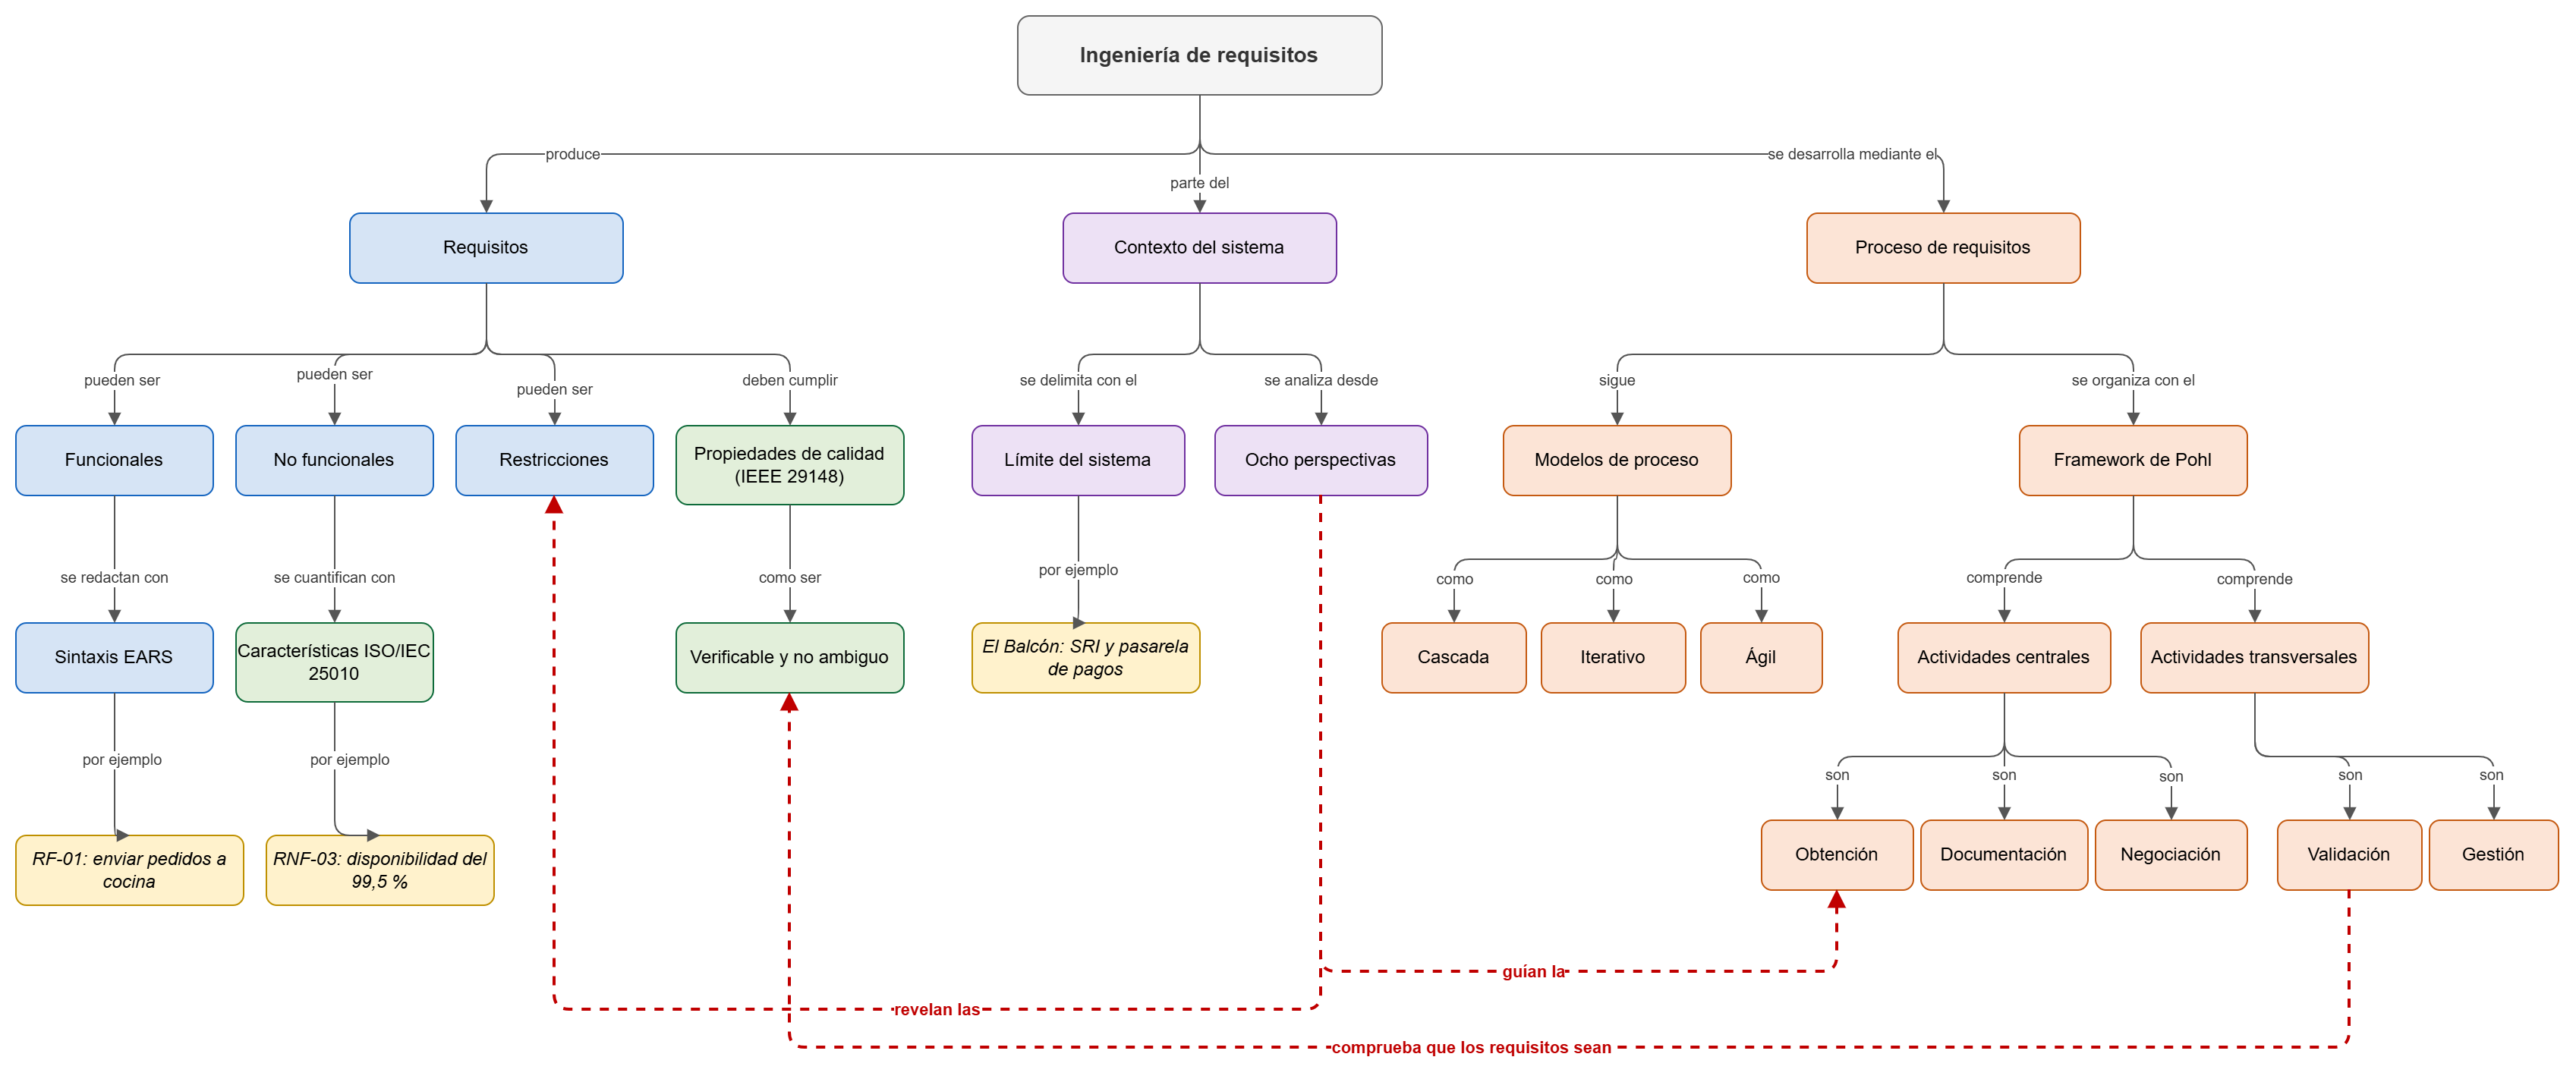
\includegraphics[width=\linewidth,height=0.85\textheight,keepaspectratio]{figuras/mapa-conceptual.png}
\caption{Mapa conceptual integrador de la Unidad 1. Elaborado en draw.io.}
\label{fig:mapa-conceptual}
\end{figure}
\end{landscape}


\section{Conclusiones}
% Responsable: Danela (1), Tahiny (2), Anthony (2) · Ronda 4 (domingo 15, hasta 15.00)
% Cinco conclusiones de mínimo 80 palabras: (1) afirmación, (2) evidencia con cita, (3) implicación para el PFC o la profesión.

% Chavarria Tahiny
\textbf{Conclusi\'on (Tahiny Chavarr\'ia, 1).} Distinguir los requisitos de sistema de los de software evita asignar al c\'odigo responsabilidades que corresponden al conjunto de hardware, software y personas. Las normas 29148, 15288 y 12207 describen una derivaci\'on por niveles, desde el stakeholder hasta el componente de software, que exige trazabilidad entre ellos \cite{iso29148,iso15288,ieee12207}. En el SGR-IA de El Balc\'on, el objetivo RN-01 de reducir mermas se traza hasta el pron\'ostico RF-02 y hasta su meta de calidad RNF-05, y as\'i el equipo sabe por qu\'e existe cada requisito y qu\'e debe revisar si cambia. Para la profesi\'on, esta trazabilidad es lo que permite gestionar el cambio sin perder el v\'inculo con las necesidades del cliente.

\textbf{Conclusi\'on (Tahiny Chavarr\'ia, 2).} Un modelo de calidad convierte adjetivos vagos en requisitos que se pueden probar. ISO/IEC 25010:2023 organiza la calidad del producto en nueve caracter\'isticas \cite{iso25010}, y Glinz advierte que, sin esa precisi\'on, los requisitos ``no funcionales'' se interpretan de forma inconsistente \cite{glinz2007}. En El Balc\'on, ``que sea r\'apido'' se transform\'o en RNF-01, con m\'etrica, umbral y condici\'on de carga, y se justific\'o por qu\'e mantenibilidad y flexibilidad quedan fuera de esta versi\'on. Para la profesi\'on, esto significa que la calidad se negocia con el cliente antes de programar y se verifica con pruebas, no con opiniones.


\textbf{Conclusión (Anthony Naranjo, 1).}
La definición del límite y del contexto del sistema permite comprender que los requisitos no surgen únicamente de las funciones que se desea programar, sino también de las personas, procesos y condiciones externas que influyen sobre la solución. El framework de Pohl considera el contexto como parte fundamental de la Ingeniería de Requisitos y propone perspectivas para analizarlo sistemáticamente \cite{pohl2025}. En El Balcón Restaurant, este análisis permitió diferenciar las funciones internas del SGR-IA de actores como el propietario, los usuarios, los clientes y servicios externos. Para
el PFC, esta delimitación reduce ambigüedades de alcance y proporciona una base más sólida para especificar requisitos verificables y mantener la coherencia del proyecto.

\textbf{Conclusión (Anthony Naranjo, 2).}
La aplicación de un proceso estructurado de Ingeniería de Requisitos permite transformar las necesidades de un negocio real en artefactos que pueden ser revisados, negociados, validados y gestionados durante el desarrollo. Pohl
organiza este trabajo mediante las actividades centrales de elicitación, documentación y negociación, apoyadas transversalmente por la validación y la gestión \cite{pohl2025}. En el caso de El Balcón Restaurant, estas
actividades permiten relacionar los problemas actuales de pedidos e inventario con requisitos concretos y con las funciones de inteligencia artificial propuestas. Para la profesión, aplicar este proceso ayuda a reducir decisiones basadas en supuestos y mantiene el desarrollo vinculado con las necesidades reales del cliente.


\printbibliography[title={Referencias}]

\appendix
\renewcommand{\thesection}{\Alph{section}}
\section{Lista de referencias exportada}
% Responsable: Danela · Ronda 4 (domingo 15, hasta 15.00)
% Anexo A: lista de referencias IEEE exportada desde Zotero o Mendeley.



\section{Biblioteca de referencias en el gestor bibliográfico}
% Responsable: Danela · Ronda 4 (domingo 15, hasta 15.00)
% Anexo B: captura de pantalla de la biblioteca en Zotero o Mendeley (figuras/anexo-b-biblioteca.png).



\section*{Declaración de uso de inteligencia artificial}
% Responsable: Danela · Cierre (domingo 15, hasta 21.00)
% Declaración de uso de IA de los tres integrantes.

% Chavarria Tahiny 
\section*{Declaraci\'on de uso de inteligencia artificial: Tahiny Mel Chavarr\'ia Cuenca}

Se us\'o Claude, asistente de inteligencia artificial de Anthropic, el 12 de noviembre de 2026, solo en mis partes del trabajo. La IA se us\'o para:

\begin{itemize}[nosep]
  \item redactar un borrador de las secciones 2.3 (requisitos de sistema y de software) y 2.4 (modelo de calidad ISO/IEC 25010:2023);
  \item proponer el diseño de la tabla de 15 requisitos de El Balc\'on Restaurant, con su tipo, redacci\'on EARS, prioridad MoSCoW y fuente;
  \item redactar un borrador de mis dos conclusiones;
  \item preparar las entradas BibTeX de las referencias y la estructura de los archivos LaTeX.
\end{itemize}


\end{document}
